%% Follow comments to support use.

%%%%%%%%%%%%%%%%%%%%%%%%%%%%%%%%%%%%%%%%%%%%%%%%%%%%%%%%%
%% STEP 1: Choose options for MSc / BSc / seminar layout and your bibliographic style
%%%%%%%%%%%%%%%%%%%%%%%%%%%%%%%%%%%%%%%%%%%%%%%%%%%%%%%%%

%%  Language: 
%%      finnish, swedish, or english
%%  Pagination (use twoside by default)  
%%      oneside or twoside,
%%  Study programme / kind of report
%%      csm  = Master's thesis in Computer Science Master's Programme;
%%      tkt = Bachelor's thesis in Computer Science Bachelor's Programme;
%%      seminar = seminar report
%%  For Master's thesis choose your line or track:
%%      (30 cr thesis, 2020 onwards, Master's Programme in Computer Science = csm)
%%      software-track-2020 = Software study track
%%      algorithms-track-2020 = Algorithms study track
%%      networking-track-2020 = Networking study track

\documentclass[english,twoside,censored,csm,algorithms-track-2020]{HYthesisML} 


% If wanted, open new chapters only at right page.
% By default, "openany".
%\PassOptionsToClass{openright,twoside,a4paper}{report}
\PassOptionsToClass{openany,twoside,a4paper}{report}

\usepackage{csquotes}
%%%%%%%%%%%%%%%%%%%%%%%%%%%%%%%%%%%%%%%%%%%%%%%%%%%%%%%%%
%% REFERENCES
%% Some notes on bibliography usage and options:
%% natbib -> you can use, e.g., \citep{} or \parencite{} for (Einstein, 1905); with APA \cite -> Einstein, 1905 without ()
%% maxcitenames=2 -> only 2 author names in text citations, if more -> et al. is used
%% maxbibnames=99 as no great need to suppress the biliography list in a thesis
%% for more information see biblatex package documentation, e.g., from https://ctan.org/pkg/biblatex 

%% Reference style: select one 
%% for APA = Harvard style = authoryear -> (Einstein, 1905) use:
\usepackage[style=authoryear,bibstyle=authoryear,backend=biber,natbib=true,maxnames=99,maxcitenames=2,uniquelist=minyear,giveninits=true,uniquename=mininit,safeinputenc]{biblatex}
%% for numeric = Vancouver style -> [1] use:
%\usepackage[style=numeric,bibstyle=numeric,backend=biber,natbib=true,maxbibnames=99,giveninits=true,uniquename=init]{biblatex}
%% for alpahbetic -> [Ein05] use:
%\usepackage[style=alphabetic,bibstyle=alphabetic,backend=biber,natbib=true,maxbibnames=99,giveninits=true,uniquename=init]{biblatex}
%

\addbibresource{thesis.bib}
% in case you want the final delimiter between authors & -> (Einstein & Zweistein, 1905) 
% \renewcommand{\finalnamedelim}{ \& }
% List the authors in the Bibilipgraphy as Lastname F, Familyname G,
\DeclareNameAlias{sortname}{family-given}
% remove the punctuation between author names in Bibliography 
%\renewcommand{\revsdnamepunct}{ }


%% Block of definitions for fonts and packages for picture management.
%% In some systems, the figure packages may not be happy together.
%% Choose the ones you need.

%\usepackage[utf8]{inputenc}  % For UTF8 support, in some systems. Use UTF8 when saving your file.


\usepackage{lmodern}         % Font package, again in some systems.
\usepackage{textcomp}        % Package for special symbols
\usepackage[pdftex]{color, graphicx} % For pdf output and jpg/png graphics
\usepackage{epsfig}
\usepackage{subfigure}
\usepackage[pdftex, plainpages=false]{hyperref} % For hyperlinks and pdf metadata
\usepackage{fancyhdr}        % For nicer page headers
\usepackage{tikz}            % For making vector graphics (hard to learn but powerful)
%\usepackage{wrapfig}        % For nice text-wrapping figures (use at own discretion)
\usepackage{amsmath, amssymb} % For better math
\usepackage{algorithm}       % For pseudocode
\usepackage[noend]{algorithmic} % For pseudocode
\usepackage{booktabs}        % For nicer tables
\usepackage{cleveref}        % For easier referencing

\usepackage{amsthm}          % Theorems
\newtheorem{theorem}{Theorem}[chapter]
\newtheorem{lemma}[theorem]{Lemma}
\newtheorem{corollary}[theorem]{Corollary}
\newtheorem{proposition}[theorem]{Proposition}
\newtheorem{exercise}[theorem]{Exercise}
\newtheorem{definition}[theorem]{Definition}
\newtheorem{conjecture}[theorem]{Conjecture}
\newtheorem{observation}[theorem]{Observation}
\theoremstyle{definition}
\newtheorem{example}[theorem]{Example}
\theoremstyle{remark}
\newtheorem{note}[theorem]{Note}
\newtheorem*{note*}{Note}
\newtheorem{remark}[theorem]{Remark}
\newtheorem*{remark*}{Remark}


% TODO Macro
\newcommand{\TODO}[1]{\textcolor{red}{#1}}

\singlespacing               %line spacing options; normally use single

\fussy
%\sloppy                      % sloppy and fussy commands can be used to avoid overlong text lines
% if you want to see which lines are too long or have too little stuff, comment out the following lines
% \overfullrule=1mm
% to see more info in the detailed log about under/overfull boxes...
% \showboxbreadth=50 
% \showboxdepth=50



%%%%%%%%%%%%%%%%%%%%%%%%%%%%%%%%%%%%%%%%%%%%%%%%%%%%%%%%%
%% STEP 2:
%%%%%%%%%%%%%%%%%%%%%%%%%%%%%%%%%%%%%%%%%%%%%%%%%%%%%%%%%
%% Set up personal information for the title page and the abstract form.
%% Replace parameters with your information.
\title{MaxSAT-Based Bi-Objective Boolean Optimization}

\author{Christoph Jabs}
\date{\today}

% Set supervisors, use the titles according to the thesis language
% in English Prof. or Dr., or in Finnish toht. or tri or FT, TkT, Ph.D. or in Swedish... 
\supervisors{Prof.~M.~J\"arvisalo, Dr.~J.~Berg, Dr.~A.~Niskanen}

\keywords{Multi-objective optimization, bi-objective optimization, maximum satisfiability, incremental SAT}
\additionalinformation{\translate{\track}}

%% For seminar reports:
%%\additionalinformation{Name of the seminar}

%% Provide classification terms, to appear on the abstract page.
%% Replace the classification terms below with the ones that match your work.
%% ACM Digital library provides a taxonomy and a tool for classification
%% in computer science. Use 1-3 paths, and use right arrows between the
%% about three levels in the path; each path requires a new line.

\classification{\protect{\ \\
\  Mathematics of computing $\rightarrow$ Discrete mathematics $\rightarrow$ Combinatorics $\rightarrow$ Combinatorial optimization \\
\  Theory of computation  $\rightarrow$ Logic $\rightarrow$ Constraint and logic programming
}}

%% If you want to quote someone special. You can comment this line out and there will be nothing on the document.
%\quoting{Bachelor's degrees make pretty good placemats if you get them laminated.}{Jeph Jacques}


%% OPTIONAL STEP: Set up properties and metadata for the pdf file that pdfLaTeX makes.
%% Your name, work title, and keywords are recommended.
\hypersetup{
    unicode=true,           % to show non-Latin characters in Acrobat’s bookmarks
    pdftoolbar=true,        % show Acrobat’s toolbar?
    pdfmenubar=true,        % show Acrobat’s menu?
    pdffitwindow=false,     % window fit to page when opened
    pdfstartview={FitH},    % fits the width of the page to the window
    pdftitle={},            % title
    pdfauthor={Christoph Jabs}, % author
    pdfsubject={},          % subject of the document
    pdfcreator={},          % creator of the document
    pdfproducer={pdfLaTeX}, % producer of the document
    pdfkeywords={algorithms}, % list of keywords for
    pdfnewwindow=true,      % links in new window
    colorlinks=true,        % false: boxed links; true: colored links
    linkcolor=black,        % color of internal links
    citecolor=black,        % color of links to bibliography
    filecolor=magenta,      % color of file links
    urlcolor=cyan           % color of external links
}

%%-----------------------------------------------------------------------------------

\newcommand{\formula}{F}
\newcommand{\Obj}{\textsc{O}}
\newcommand{\inc}{\text{I}}
\newcommand{\dec}{\text{D}}
\newcommand{\var}{\textsc{var}}
\newcommand{\lit}{\textsc{lit}}
\newcommand{\Min}{\texttt{Minimize-\allowbreak{}Inc}}
\newcommand{\Simpr}{\texttt{Solution-\allowbreak{}Improving-\allowbreak{}Search}}
\newcommand{\E}{\texttt{EnumSols}}
\newcommand{\Ex}{\texttt{ExistsSol}}
\newcommand{\T}{\mathtt{T}}
\newcommand{\assumps}{\mathcal{A}}
\newcommand{\satsolver}{\texttt{isSAT}}
\newcommand{\res}{\text{res}}
\newcommand{\algname}{\textsc{BiOptSat}}
\newcommand{\tot}{\textsc{Tot}}
\newcommand{\ov}[2]{\langle #1 < #2 \rangle}
\newcommand{\ove}[2]{\langle #1 \leq #2 \rangle}
\newcommand{\satunsat}{\texttt{SAT-\allowbreak{}UNSAT}}
\newcommand{\unsatsat}{\texttt{UNSAT-\allowbreak{}SAT}}
\newcommand{\msu}{\texttt{MSU3}}
\newcommand{\I}{\mathcal{I}}
\newcommand{\Act}{\texttt{Act}}
\newcommand{\oll}{\texttt{OLL}}
\newcommand{\msh}{\texttt{MSHybrid}}
\newcommand{\hs}{\texttt{hs}}
\newcommand{\nsamp}{n}
\newcommand{\nfeat}{m}
\newcommand{\nclauses}{k}
\newcommand{\selector}{s}
\newcommand{\noise}{\eta}
\newcommand{\equals}{e}
\newcommand{\nelems}{n}
\newcommand{\nsets}{m}
\newcommand{\setcard}{s}
\newcommand{\elemprob}{p}
\newcommand{\sets}{\mathcal{S}}
\newcommand{\element}{e}
\newcommand{\cover}{\mathcal{C}}
\newcommand{\cost}{c}
\newcommand{\cores}{\mathcal{K}}
\newcommand{\core}{\kappa}
\newcommand{\sol}{\tau}
\newcommand{\scep}{SetCovering-EP}
\newcommand{\scsc}{SetCovering-SC}
\newcommand{\clause}{C}
\newcommand{\softs}{\textsc{S}}
\newcommand{\generalobj}{f}
\newcommand{\nobj}{p}
\newcommand{\feasible}{\mathcal{X}}
\newcommand{\decvar}{x}
\newcommand{\soloone}{\{i_2,\allowbreak d_1,\allowbreak d_3,\allowbreak d_4,\allowbreak \lnot i_1,\allowbreak \lnot i_3,\allowbreak \lnot i_4,\allowbreak \lnot d_2\}}
\newcommand{\solotwo}{\{i_1,\allowbreak i_2,\allowbreak d_1,\allowbreak d_2,\allowbreak \lnot i_3,\allowbreak \lnot i_4,\allowbreak \lnot d_3,\allowbreak \lnot d_4\}}
\newcommand{\solothree}{\{i_2,\allowbreak d_1,\allowbreak d_3,\allowbreak d_4,\allowbreak \lnot i_1,\allowbreak \lnot i_3,\allowbreak \lnot i_4,\allowbreak \lnot d_2\}}
\newcommand{\solcone}{\{i_1,\allowbreak i_2,\allowbreak i_3,\allowbreak i_4,\allowbreak d_1,\allowbreak d_2,\allowbreak d_3,\allowbreak d_4\}}
\newcommand{\solctwo}{\{i_1,\allowbreak i_2,\allowbreak d_1,\allowbreak d_2,\allowbreak d_3,\allowbreak d_4,\allowbreak \lnot i_3,\allowbreak \lnot i_4\}}
\newcommand{\solcthree}{\{i_2,\allowbreak d_1,\allowbreak d_2,\allowbreak d_3,\allowbreak d_4,\allowbreak \lnot i_1,\allowbreak \lnot i_3,\allowbreak \lnot i_4\}}
\newcommand{\solcfour}{\{i_1,\allowbreak i_2,\allowbreak i_3,\allowbreak d_1,\allowbreak d_2,\allowbreak \lnot i_4,\allowbreak \lnot d_3,\allowbreak \lnot d_4\}}
\newcommand{\solmcstrap}{\{i_1,\allowbreak i_3,\allowbreak i_4,\allowbreak d_1,\allowbreak d_3,\allowbreak d_4,\allowbreak \lnot i_2,\allowbreak \lnot d_2\}}
\newcommand{\TODO}[1]{\textcolor{red}{#1}}
\newcommand{\thr}{\texttt{thr}}
\newcommand{\NP}{$\mathcal{NP}$}

\begin{document}

% Generate title page.
\maketitle

%%%%%%%%%%%%%%%%%%%%%%%%%%%%%%%%%%%%%%%%%%%%%%%%%%%%%%%%%
%% STEP 3:
%%%%%%%%%%%%%%%%%%%%%%%%%%%%%%%%%%%%%%%%%%%%%%%%%%%%%%%%%
%% Write your abstract in the separate file, to be positioned here.
%% You can make several abstract pages (if you want it in different languages),
%% in which case you should also define the language of the abstract,
%% as below.

\include{Ch.00_Abstract}

% Place ToC
%\newpage
\mytableofcontents

\mainmatter

%%%%%%%%%%%%%%%%%%%%%%%%%%%%%%%%%%%%%%%%%%%%%%%%%%%%%%%%%
%% STEP 4: Write the thesis.
%%%%%%%%%%%%%%%%%%%%%%%%%%%%%%%%%%%%%%%%%%%%%%%%%%%%%%%%%
%% Your actual text starts here. You shouldn't mess with the code above the line except
%% to change the parameters. Removing the abstract and ToC commands will mess up stuff.
%%
%% Command \include{file} includes the file of name file.tex.
%% A new page will be created at every \include command, 
%% which makes it appropriate to use it for large entities such as book chapters. Cannot be nested.
%% It is useful for a big project, as changing one of the include targets 
%% won't force the regeneration of the outputs of all the rest.
%% Alternatively, \input is a more lower level macro 
%% which simply inputs the content of the given file like it was copy&pasted there manually.

\chapter{Introduction\label{chap:intro}}


\chapter{Preliminaries\label{chap:preliminaries}}

In this chapter, an overview of subjects that this work builds on is given.
The first section discusses propositional satisfiability, as this is the declarative paradigm the presented algorithm builds on.
Following that, bi-objective optimization is described, starting from a general perspective and ending up with notation used for bi-objective optimization in the context of propositional logic.
The chapter is concluded with a section overviewing different approaches to solving bi-objective optimization problems.
The focus hereby is on approaches based on propositional satisfiability, but others are briefly discussed as well.

\section{Propositional Satisfiability\label{sec:sat}}

For a Boolean variable $x$ there are two literals, the positive $x$ and the negative $\lnot x$. 
A clause $C$ is a set of (disjunction over) literals and a CNF formula $\formula$ is a set of (conjunction over) clauses.
A truth assignment $\sol$ maps boolean variables to $1$ (true) or $0$ (false).
The semantics of truth assignments are extended to a clause $C$ and a formula $\formula$ in the standard way: $\sol(C) = \max\{ \sol(l) \mid l \in C\}$ and $\sol(\formula) = \min\{\sol(C) \mid C \in \formula\}$.
When convenient, we view assignments $\sol$ over a set $X$ of variables as sets of literals $\sol = \{ x \mid x \in X,  \sol(x) = 1\} \cup \{ \lnot x \mid x \in X, \sol(x) = 0\}$.
An assignment $\sol$ for which $\sol(\formula) = 1$ is a solution to $\formula$.
The set of variables and literals appearing in $\formula$ are $\var(\formula)$ and $\lit(\formula)$, respectively.  
The propositional satisfiability (SAT) problem asks whether for a given formula $\formula$, a solution exists.
A formula $\formula$ is satisfiable if it has solutions, otherwise it is unsatisfiable.
\begin{example}
  Take the propositional formula $\formula_1 = a \land \lnot b$ over variables $\var(\formula_1) = \{a,b\}$.
  It is satisfiable since the assignment $\sol=(a,\lnot b)$ has $\sol(\formula_1)=1$.
  The formula $\formula_2 = a \land \lnot a$ on the other hand is not satisfiable since no assignment $\sol$ with $\sol(\formula_2)=1$ exists.
\end{example}

A SAT solver is an algorithm that solves the SAT problem for a given formula $\formula$.
If the formula is satisfiable, it returns ``satisfiable'' (SAT) and a solution $\sol$ with $\sol(\formula)=1$;
if it is unsatisfiable, it return ``unsatisfiable'' (UNSAT).

The SAT problem was proved $\mathcal{NP}$-complete in~\textcite{DBLP:conf/stoc/Cook71}.
This result is very central to its modern day use as a declarative programming approach to solving other $\mathcal{NP}$-complete problems by encoding them as a propositional formula first, solving them with a SAT solver and then decoding the solution to the original problem context.
The advantage of using SAT as a declarative programming language for solving other problems comes from the fact that---even though SAT is $\mathcal{NP}$-complete, and it is unclear if a polynomial time algorithm for solving it exists---conflict-driven clause learning solvers~\autocite{handbook2-cdcl} for SAT are efficient in practice and can solve problems with hundred-thousands of variables and clauses \TODO{check claim}.
\begin{example}
  Consider the problem of whether to wear tie and shirt to a given event with the following constraints:
  (i)~one should not wear a tie without a shirt, (ii)~not wearing a tie nor a shirt is impolite, and (iii)~wearing a shirt and a tie is considered overdressed.
  To solve this problem with the help of SAT, it can be encoded to propositional logic by introducing variables $v_\text{shirt}$ and $v_\text{tie}$ that represent if a shirt or a tie is worn.
  The constraint can then be encoded as the following clauses:
  $\clause_\text{(i)} = \lnot v_\text{tie} \lor v_\text{shirt}$, $\clause_\text{(ii)} = v_\text{tie} \lor v_\text{shirt}$ and $\clause_\text{(iii)} = \lnot v_\text{tie} \lor \lnot v_\text{shirt}$.
  The formula $\clause_\text{(i)} \land \clause_\text{(ii)} \land \clause_\text{(iii)}$ can then be solved with a SAT solver, which will return the satisfying assignment $\{ v_\text{shirt}, \lnot v_\text{tie} \}$.
  This solution is decoded as it being appropriate to wear a shirt but no tie.
  \TODO{can I use this example?}
\end{example}

In this work, w.l.o.g.\ we assume that all formulas are satisfiable \TODO{relevant?}.

\subsection{Incremental SAT Solving under Assumptions\label{sec:inc-sat}}

It is common that algorithms that solve problems with the help of SAT solvers produce a series of SAT problems that only differ slightly.
To be able to solve these subproblems more efficiently, most modern SAT solvers provide an incremental interface that allows for retaining information learned in previous solver calls \TODO{check if new CDCL chapter can be referenced}.
In order for the learned information from previous solver queries to still hold for subsequent calls, it is only possible to add clauses to the solvers internal formula, not remove them.
In addition, incremental SAT solvers support solving under assumptions.
The assumptions $\assump$ are a set of literals that are treated as unit clauses, i.e.\ a solver call with internal formula $\formula$ and assumptions $\assump$ either returns SAT and a solution $\sol \supset \assump$, or UNSAT and a subset $\core \subset \{\lnot l \mid l\in\assump\}$ such that $\formula \land \bigwedge_{l \in \core} (\lnot l)$ is unsatisfiable.
The subset $\core$ is called an unsatisfiable \emph{core} and, intuitively, is an explanation for the unsatisfiability of the query.

\subsection{Maximum Satisfiability\label{sec:max-sat}}

Maximum satisfiability (MaxSAT) is the optimization variant of the decision SAT problem.
In it, the goal is to find a solution that satisfies as many of the given clauses as possible.
Most commonly and in this work, MaxSAT refers to the extension of weighted partial MaxSAT, in which a set of \emph{hard} clauses $\formula$ and another set of \emph{soft} clauses $\softs$ are given.
Each clause $\clause \in \softs$ is assigned a weight $w_\clause$ and a solution $\sol$ that satisfies $\formula$ while minimizing $\sum_{\clause\in\softs \mid \tau(\clause)=0} w_\clause$ is optimal for the problem.

In the same way that SAT can be used as a declarative language to solve other decision problems, MaxSAT can be used to solve other optimization problems.

\subsection{Encoding Cardinality Constraints\label{sec:card-const}}

A common type of constraint to appear when encoding problems into SAT is that of a cardinality constraint.
Cardinality constraints, informally speaking, enforce a bound on how many literals in a set can be assigned to true.
Formally, for a set $L$ of literals and a bound $k \in \mathbb{N}$, $\texttt{As-CNF}\left(\sum_{l \in L} l \circ k\right)$ denotes a CNF formula that encodes the linear inequality $\sum_{l \in L} l \circ k$, where $\circ \in \{ ,< ,> ,\geq, \leq, =\}$.
Numerous methods of forming such CNF formulas are known~\autocite{DBLP:conf/cp/BailleuxB03}.
In this work we make use of the totalizer encoding.

Given a set $L$ of $n$ input literals and a bound $k=1, \ldots, n$, the (incremental) totalizer~\autocite{DBLP:conf/cp/BailleuxB03,DBLP:conf/cp/MartinsJML14} encoding produces a CNF formula $\tot(L, k)$ that defines a set $\{\ov{L}{1}, \ldots, \ov{L}{k}\} \subset \var(\tot(L))$ of \emph{output literals} that---informally speaking---count the number of literals in $L$ assigned to true by solutions to $\tot(L)$:
if $\tau$ is an assignment that satisfies $\tot(L)$, then $\tau(\ov{L}{b}) = 1$ if $\sum_{l \in L} \tau(l) < b$ \TODO{point out that iff (or $\leftarrow$) are possible as well, but we only need upper bounds)}.
The incremental totalizer supports both increasing the bound $k$ and adding new input literals without having to rebuild the whole formula:
we have that $\tot(L, k) \subset \tot(L, k')$ and $\tot(L, k) \subset  \tot(L \cup L', k)$ hold for any bound $k' > k$ and set $L'$ of literals for which $L \cap L' =  \emptyset$. 
We use $\ove{L}{k}$ as a shorthand for the literal $\ov{L}{k+1}$.
We note that the assignments of the auxiliary variables of the totalizer encoding are functionally defined by the assignment of the input and output variables.
As such we will leave them out from the solutions we describe in favour of brevity and clarity of examples. 

\section{Bi-Objective Optimization\label{sec:biopt}}

\TODO{General bi-opt setting}

An objective $\Obj$ is a multiset of literals, which allows for representing objective functions with non-unit coefficients.
The value $\Obj(\tau)$ of a truth assignment $\tau$ under $\Obj$ is $\Obj(\tau) = \sum_{l \in \Obj} \tau(l)$, i.e., the number of the literals in $\Obj$ that $\tau$ assigns to $1$. 
Weighted objectives can be represented by adding a literal multiple times.
% Note that formulating the optimization task in terms of minimizing the number of literals set to true by a truth assignment is equivalent to maximum satisfiability (MaxSAT). \TODO{somethign missing, at least a CNF?}

 %It also makes our algorithm applicable for solving bi-objective constrained optimization problems~\cite{DBLP:conf/aaai/HartertS14,DBLP:conf/cp/SohBTB17,DBLP:conf/sat/Terra-NevesLM17} by encoding  them into CNF.

Given a CNF formula $\formula$, two objectives $\Obj_1, \Obj_2 \subset \lit(\formula)$ and solutions $\tau_1, \tau_2$ to $\formula$, we say that $\tau_1$ dominates $\tau_2$ if (i)~$\Obj_i(\tau_1) \leq \Obj_i(\tau_2)$ for $i=1,2$, and (ii)~either $\Obj_1(\tau) < \Obj_1(\tau_2)$  or $\Obj_2(\tau) < \Obj_2(\tau_2)$.
A solution $\tau$ is pareto-optimal if no other solution dominates it.
The pareto front of $\formula$ w.r.t.\ $\Obj_1, \Obj_2$ consists of all solutions of $\formula$ that are pareto-optimal w.r.t.\ $\Obj_1$ and $\Obj_2$. 
When the objectives are clear from context, we will simply say that a solution $\tau$ is a pareto-optimal solution of $\formula$. 
The pair $(\Obj_1(\tau),\Obj_2(\tau))$ of a pareto-optimal $\tau$ is a pareto point (of $\formula$ w.r.t.\ $\Obj_1$ and $\Obj_2$).
Note that there may be multiple solutions that correspond to the same pareto point.
We consider the task of computing a representative solution for each pareto point as well as the task of enumerating all solutions in the pareto front.

\begin{figure}
  \begin{minipage}{0.36\textwidth}
  \footnotesize
  \begin{align*}
  \formula = &\{ \texttt{As-CNF}\left(\sum_ {x \in \Obj_\inc \cup \Obj_\dec} x \geq 3 \right), \\
  			&(i_1 \lor i_2),  (i_2 \lor i_3), \\
		 &(d_1 \lor d_2), (d_2 \lor d_3) \} \\ \\
  \Obj_\dec =&\{ d_1,d_2, d_3\}   \\ 
  \Obj_\inc =&\{ i_1,i_2, i_3\}  
  \end{align*}
  \end{minipage}
  \;
  \begin{minipage}{0.6\textwidth}
    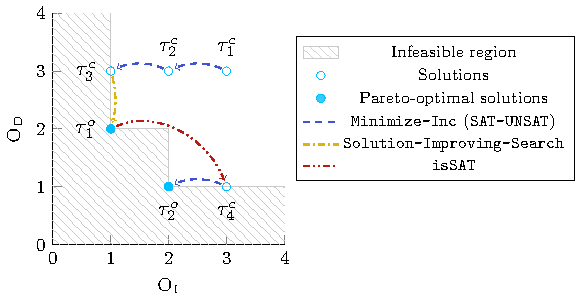
\includegraphics{search-trace.pdf}
  \end{minipage}
  \caption{Left: An example formula $\formula$ and two objectives $\Obj_\inc$ and $\Obj_\dec$.
    Right: the solution space of $\formula$ w.r.t.\ $\Obj_\inc$ and $\Obj_\dec$.
    The solutions $\tau^o_1$ and $\tau^o_2$ (solid points) are pareto-optimal, while $\tau^c_i$ for $i=1,\ldots,4$ are not.\label{fig:search-trace}}
\end{figure}

\begin{example}\label{ex:main}
  An example formula $\formula$ and two objectives $\Obj_\inc$ and $\Obj_\dec$ are shown on the left side of \cref{fig:search-trace}. 
  The solution space is illustrated on the right.
  The two solid dots correspond to the two pareto points of $\formula$ w.r.t.\ $\Obj_\inc$ and $\Obj_\dec$. 
  Examples of pareto-optimal solutions corresponding to these points are $\tau^o_1 = \{d_1, d_3, i_2, \lnot d_2, \lnot i_1, \lnot i_3\}$ and $\tau^o_2 = \{i_1, i_3, d_2, \lnot i_2, \lnot d_1, \lnot d_3\}$.
\end{example}

An important property of pareto-optimal solutions to bi-objective problems is summarized by the next proposition.

\begin{proposition}[Adapted from~\autocite{DBLP:conf/aaai/HartertS14}] \label{prop:biobjective}
  Sorting the pareto-optimal solutions of $\formula$ w.r.t.\ increasing values of $\Obj_1$ is equivalent to sorting them w.r.t.\ decreasing values of $\Obj_2$ and vice-versa.
\end{proposition}

\begin{example}
  Consider the formula $\formula$, the objectives $\Obj_\inc$ and $\Obj_\dec$ and the two pareto-optimal solutions $\tau^o_1$ and $\tau^o_2$ from \cref{fig:search-trace} and \cref{ex:main}.
  By the definition of pareto-optimality, lowering the value of one objective of a pareto-optimal solution has to increase the value of the other;
  we have $\Obj_\inc(\tau^o_1) = 1 < 2 = \Obj_\inc(\tau^o_2)$ and $\Obj_\dec(\tau^o_1) = 2 > 1 = \Obj_\dec(\tau^o_2)$.
\end{example}

\section{Approaches to Bi-Objective Optimization\label{sec:approaches}}

\TODO{signposting}

\subsection{SAT-Based Approaches\label{sec:sat-based}}

\subsubsection{$P$-minimal Solution Enumeration\label{sec:p-minimal}}

The approach perhaps closest to ours is solving multi-objective constraint optimization problems by enumerating so-called $P$-minimal solutions~\autocite{DBLP:conf/cp/SohBTB17,DBLP:conf/ftp/KoshimuraNFH09}.
We were unable to obtain an implementation of the approach from the authors.
For a fair comparison with \algname{}, we hence reimplemented the approach similarly as \algname{}.
In more detail, the $P$-minimal approach  corresponds to enumerating the solutions of $\formula^\text{W} = \formula \land \tot(\Obj_{\inc}) \land \tot(\Obj_{\dec})$ that are subset-minimal w.r.t.\ the set of outputs of the totalizers.
More precisely, if $P$ is the set of output literals of $\tot(\Obj_{\inc}) \land \tot(\Obj_{\dec})$, then the goal is to enumerate solutions $\tau_m$ such that no other solution $\tau$ has $\{ b \mid b \in P \land \tau(b) = 0\} \subsetneq \{ b \mid b \in P \land \tau_m(b) = 0\}$.
The procedure for enumerating such solutions (detailed in~\textcite{DBLP:conf/ftp/KoshimuraNFH09}) works by (i)~using a solver to obtain any solution $\tau$ of $\formula^\text{W}$, (ii)~iteratively minimizing the subset of variables of $P$ set to true by the solution, and, once a minimal solution $\tau_m$ has been found, (iii)~adding the clause $(\ov{\Obj_{\inc}}{k_1} \lor \ov{\Obj_{\dec}}{k_2})$ containing the output variables corresponding to the lowest index set to true by $\tau_m$.

\begin{example}
  Consider the formula $\formula$ and two objectives $\Obj_\inc$ and $\Obj_\dec$ from \cref{fig:search-trace}.
  $P$-minimal starts by building two totalizers $\tot(\Obj_\inc)$ and $\tot(\Obj_\dec)$ and invoking the SAT solver on $\formula^\text{W} = \formula \land \tot(\Obj_\inc) \land \tot(\Obj_\dec)$.
  The result is satisfiable, assume the first solution obtained is $\tau^c_1 = \{i_1, i_2, i_3, d_1, d_2, d_3\}$. 
  In order to minimize $\tau^c_1$, the clause $(\ov{\Obj_\inc}{3} \lor \ov{\Obj_\dec}{3})$ is added to the SAT solver, and the solver is invoked again under the assumptions $\{ \ove{\Obj_\inc}{3}, \ove{\Obj_\dec}{3} \}$.
  The added clause blocks $\tau^c_1$ and all solutions dominated by $\tau^c_1$ from the search space.
  Assume the next solution obtained is $\tau^c_5 = \{d_1, d_3, i_1, i_3, \lnot d_2, \lnot i_2\}$. 
  Again, a clause $(\ov{\Obj_\inc}{2} \lor \ov{\Obj_\dec}{2})$ is added, and the SAT solver is queried with assumptions $\{ \ove{\Obj_\inc}{2}, \ove{\Obj_\dec}{2} \}$.
  The result is SAT, assume the solution obtained is $\tau^o_2 = \{ i_1, i_3, d_2, \lnot i_2, \lnot d_2, \lnot d_3\}$. 
  $P$-minimal then adds the clause $(\ov{\Obj_\inc}{2} \lor \ov{\Obj_\dec}{1})$ and invokes the solver again under the assumptions $\{ \ove{\Obj_\inc}{2}, \ove{\Obj_\dec}{1} \}$.
  The result is UNSAT which proves that $\tau^o_2$ is pareto-optimal. 
  To find a next pareto-optimal solution, the solver is queried without any assumptions for a new solution to start the minimization process from.
\end{example}

Note that $P$-minimal has no guarantee on the order that the solutions are enumerated in. 
Intuitively, when an intermediate solution $\tau$ is found, the following SAT solver call either provides another solution that dominates $\tau$, or proves that $\tau$ is pareto-optimal.  

%As presented in~\cite{DBLP:conf/cp/SohBTB17}, $P$-minimal will only enumerate a single solution per pareto point.
In our implementation we extended $P$-minimal to the task of enumerating all solutions on the pareto front.
Specifically, we add a new relaxation variable $r$ to the clause added each iteration for use as an assumption to enumerate all solutions at that pareto point in a standard way.
If the next solution found dominates the previous one, we harden the clause added at the previous iteration by adding $\lnot r$ as a unit clause.
Also, once all solutions for that pareto point are enumerated, the clause is hardened.

\subsubsection{Enumeration of Pareto-Minimal Correction Sets\label{sec:pareto-mcs}}

In~\textcite{DBLP:conf/ijcai/Terra-NevesLM18a,DBLP:conf/aaai/Terra-NevesLM18,DBLP:conf/ijcai/Terra-NevesLM18} an approach for computing pareto-optimal solutions via so-called pareto-minimal correction sets (paretoMCSes) was proposed.
%A paretoMCS  consists  of two sets of literals $(M_1, M_2)$  such that  (i)~$M_1 \subset \Obj_1$ and $M_2 \subset \Obj_2$, and (ii)~there is
%a pareto-optimal solution $\tau$ that sets $\tau(o) = 1$ for all $o \in M_1 \cup M_2$ and $\tau(o) = 0$ for all other $o \in (\Obj_1 \cup \Obj_2) \setminus (M_1 \cup M_2)$.
%In~\cite{DBLP:conf/ijcai/Terra-NevesLM18a}, the computation of pareto-optimal solutions is reduced into the computation of paretoMCSes.
%The  task computing paretoMCSes is  accomplished in~\cite{DBLP:conf/ijcai/Terra-NevesLM18a}
In terms of our notation, the approach works by enumerating all subsets $S \subset  (\Obj_{\inc} \cup \Obj_{\dec})$ for which (i) $\formula \land \bigwedge_{l \in  (\Obj_{\inc} \cup \Obj_\dec) \setminus S} (\lnot l)$ is satisfiable and (ii) $\formula \land \bigwedge_{l \in  (\Obj_{\inc} \cup \Obj_\dec) \setminus S'} (\lnot l)$ is unsatisfiable for all $S' \subsetneq S$.
%(i)~there is a \emph{corresponding solution} $\tau^S$ that sets $\tau^S(o) = 1$ for all $o \in S$ and $\tau(S) = 0$ for all $o \in  (\Obj_1 \cup \Obj_2) \setminus S$, and (ii)~no such solution exists for any $S' \subsetneq S$.
Let $\mathcal{S}$ be the collection of all such sets.
The computation of $\mathcal{S}$ corresponds to MCS enumeration to which numerous algorithms have been proposed~\autocite{DBLP:conf/lpar/BendikC20,DBLP:conf/hvc/MorgadoLM12,DBLP:conf/sat/PrevitiMJM17}.
The pareto-optimal solutions are obtained by extracting the solutions satisfying $\formula \land \bigwedge_{l \in  (\Obj_{\inc} \cup \Obj_\dec) \setminus S} (\lnot l)$ for all $S \in \mathcal{S}$ and removing the dominated ones~\cite{DBLP:conf/ijcai/Terra-NevesLM18a}.
The paretoMCS approach to multi-objective optimization is approximative in that it can only guarantee that a solution is pareto-optimal once the full set $\mathcal{S}$ has been computed.
In contrast, every minimal solution found during the $P$-minimal approach of~\textcite{DBLP:conf/cp/SohBTB17} and every solution returned by the $\E$ subroutine of \cref{alg:base-algorithm} is immediately known to be pareto-optimal.
\begin{example}\label{ex:MCS}
  Consider the formula $\formula$ and two objectives $\Obj_\inc$ and $\Obj_\dec$ from \cref{fig:search-trace}.
  The paretoMCS enumeration procedure will return the solution $\tau = \{d_1, d_3, i_1, i_3\}$ since no solution $\tau_s$ of $\formula$ has $\{x \in \Obj_\inc \cup \Obj_\dec \mid  \tau_s(x) = 1\} \subsetneq \{d_1, d_3, i_1, i_3\}$.
  The solution $\tau$ is not pareto-optimal, but only filtered out in the end when all solutions in $\mathcal{S}$ have been enumerated.
\end{example}
The fact that the solution $\tau$ is not pareto-optimal can only be discovered when a solution that dominates it is enumerated. 
However, there are no guarantees on when such a dominating solution is found. 

\subsubsection{Implicit Hitting Set: Seesaw\label{sec:seesaw}}

Seesaw~\autocite{DBLP:conf/cp/JanotaMSM21} was recently proposed as a framework for bi-objective optimization as a generalization of the so-called implicit hitting set approach~\autocite{DBLP:conf/cp/DaviesB13,DBLP:conf/cp/IgnatievPLM15,DBLP:conf/kr/SaikkoWJ16,DBLP:conf/cade/FazekasBB18,DBLP:conf/kr/SaikkoDAJ18}.
In contrast to our work, a main ingredient in Seesaw is the idea of treating one of the objectives as a black box.
This allows for---but also requires---problem-specific instantiations of the black box;
no generic Seesaw implementation applicable generally to bi-objective optimization is available.
That said, to enable a comparison with (an instantiation of) Seesaw, we instantiated the approach for the LIDR problem.
(For bi-objective set covering, both objectives are monotone over the chosen cover;
instantiating Seesaw is not feasible because the refined core extraction method from~\textcite{DBLP:conf/cp/JanotaMSM21} cannot be used, resulting in enumerating all possible solutions.)

While the original paper presents Seesaw in general terms, in our context the Seesaw algorithm computes pareto-optimal solutions of a formula $\formula$ by maintaining a collection $\cores$ of subsets of $\Obj_\inc$ that are called \emph{cores}.
Informally speaking, every solution $\tau$ that improves on $\Obj_\dec$ needs to assign at least one literal from each core to $1$.
The algorithm works iteratively by computing a hitting set $\hs \subset \Obj_\inc$ (using an integer programming solver, in our case CPLEX 20.10), i.e., a subset-minimal set of literals of $\Obj_\inc$ that intersects with each core in $\mathcal{C}$, and then a solution $\tau$ that sets $\tau(o) = 1$ for each $o \in \hs$ and $\tau(o) = 0$ for each $o \in \Obj_\inc \setminus \hs$ and for which $\Obj_\dec(\tau)$ is the smallest possible value for all such solutions if one exists.
The iteration then extracts a new core that $\hs$ does not intersect with.
The pareto-optimal solutions of $\formula$ are identified by the size of the hitting set increasing.
More precisely, if the hitting set is found to increase from size $|\hs|$ to size $|\hs_2|$ with $|\hs_2|>|\hs|$, the solution $\tau$ found with a hitting set of size $|\hs|$ that has the smallest minimal value $\Obj_\dec(\tau)$ is pareto-optimal~\autocite{DBLP:conf/cp/JanotaMSM21}.

We instantiated Seesaw for LIDR by using misclassifications as the objective over which cores are extracted and a hitting set $\hs$ is found with the help of CPLEX over these cores.
In the second step, the number of literals in the smallest rule misclassifying the examples in $\hs$ or a subset of it is found.
This function is implemented as a solution-improving search  in CaDiCaL.
This instantiation was chosen because finding the smallest rule misclassifying $\hs$ is an anti-monotone function and the refined version of core extraction presented in~\textcite{DBLP:conf/cp/JanotaMSM21} can therefore be used, making Seesaw feasible in the first place.

\begin{example}
  Consider the formula $\formula$ and two objectives $\Obj_\inc$ and $\Obj_\dec$ from \cref{fig:search-trace}. 
  Initially there are no cores, so $\cores = \emptyset$. As such the first hitting set $\hs = \emptyset$ will also be empty.
  Since there are no solutions $\tau$ that set $\tau(u) = 0$ for each $u \in \Obj_\inc$, the iteration ends by extracting $\Obj_\inc$ as a core. 
  The intuition here is that at this point, we know that any solution $\tau$ of $\formula$ sets at least one variable in $\Obj_\inc$ to $1$.

  In the next iteration, a hitting set over $\cores = \{ \Obj_\inc \}$ is computed. There are a number of alternatives for such hitting sets, assume $\hs = \{ i_1 \}$.
  Since there are no solutions $\tau$ of $\formula$ that set $\tau(i_2) = \tau(i_3) = 0$, the iteration ends with extracting $\{ i_2, i_3\}$ as a new core.
  At this point we know that any solution sets at least one variable of $\Obj_\inc$ and one from $\{i_2, i_3\}$ to $1$.

  Assume the next hitting set computed is $\hs = \{i_2\}$. Now there actually are solutions $\tau$ of $\formula$ that set $\tau(i_1) = \tau(i_3) = 0$, one that minimizes 
  $\Obj_\dec(\tau)$ is $\tau^o_1 = \{d_1, d_3, i_2, \lnot d_2, \lnot i_1, \lnot i_3 \}$. The iteration ends with extracting the core
  $\kappa = \{i_1, i_3\}$. Now the intuition is that, since $\tau^o_1$ minimizes $\Obj_\dec$ over solutions that assign $\tau(u) = 0$ for every $u \notin \hs$, every solution that obtains a lower value of $\Obj_\dec$
  assigns at least one literal of $\kappa$ to $1$ as well. 

  In the next iteration, the set $\cores$ of cores is $\cores = \{ \Obj_\inc, \{i_2, i_3\}, \{i_1, i_3\}\}$. The only subset minimal hitting set $\hs$ of $\cores$ is $\hs = \{i_3\}$.
  There are no solutions $\tau$ that set $\tau(i_1) = \tau(i_2) = 0$ so a new core $\{i_1, i_2\}$ is extracted. 
  In the next iteration, one possible hitting set is $\hs = \{i_1, i_3\}$. Since the size of the hitting set grew from $1$ to $2$, the algorithm concludes that $\tau^o_1$ is pareto-optimal. 
  In this iteration, the pareto-optimal solution $\tau^o_2 = \{d_2, i_1, i_3, \lnot d_1, \lnot d_3, \lnot i_2 \}$ is obtained 
  as the solution that minimizes $\Obj_\dec$ over all solutions $\tau$ that set $\tau(i_2) = 0$.  

  The algorithm continues in this manner, computing the hitting sets, $\{i_1, i_2\}$, $\{i_2, i_3\}$ and $\{i_1, i_2, i_3\}$. 
  After computing the hitting set consisting of all literals in $\Obj_\inc$, the core extracted is $\emptyset$ at which point the algorithm terminates. 
\end{example}

%Note that the core-extraction strategy that only computes $\Obj_\inc \setminus \hs$ as the new core detailed in the example corresponds to what is called the weakest possible strategy in~\cite{DBLP:conf/cp/JanotaMSM21}.
%For the comparison
%we implemented also
%the improvements to SeeSaw proposed in~\cite{DBLP:conf/cp/JanotaMSM21} as the original authors  mention that the weakest strategy essentially reduces to enumerating
%all subsets of $\Obj_\inc$, thus being infeasible in practice. 
Note that, in contrast to $\algname$ and $P$-minimal, extending Seesaw as it is presented in~\textcite{DBLP:conf/cp/JanotaMSM21} to support the enumeration of all pareto-optimal solutions seems non-trivial.
For a non-formal intuition note that, while Seesaw is guaranteed to find at least one solution obtaining the objective values of each pareto-optimal point, the non-deterministic hitting set computation might steer the algorithm past other solutions that obtain the same values.

\subsubsection{SAT-Based Lexicographic Optimization\label{sec:lex-opt}}

\subsection{Other Declarative Optimization Paradigms\label{sec:other-approaches}}

\subsection{Approximative Approaches\label{sec:approximative}}

\chapter{The Approach\label{chap:approach}}

We detail the MaxSAT-based approach to bi-objective optimization developed in this work together with its variants.

\begin{algorithm}[t]
  \caption{\algname: MaxSAT-based  bi-objective optimization} %\TODO{Alternatively ``enumeration of'', but then it sounds like full enumeration again.}}
  \label{alg:base-algorithm}
  \textbf{Input}: A formula $\formula$, two objectives $\Obj_\inc$ and $\Obj_\dec$.\\
  \textbf{Output}: Either one or all pareto-optimal solution corresponding to each pareto point of $\formula$.

  \begin{algorithmic}[1]
    \STATE $\texttt{InitSATsolver}(F)$ \label{l:init-solv} 
    \STATE $(\res, \tau) \gets \satsolver(\emptyset)$ \quad\COMMENT{Invokes the SAT solver on the formula.}  \label{l:sols} 
    \IF{$\res=\text{UNSAT}$}
      \STATE \textbf{return} ``no solutions''
    \ENDIF
    \STATE $b_\dec \gets \infty, b_\inc \gets 0$ \label{l:bounds}
    \WHILE{$\res = \text{SAT}$} \label{l:loopstart}
    \STATE $(b_\inc, \tau) \gets \Min(b_\dec , \Obj_\inc(\tau))$  \quad\COMMENT{Maintains $\tot(\Obj_\inc)$ (or similar)}\label{l:minim1}
    \STATE $(b_\dec, \tau) \gets  \Simpr(b_\inc , \Obj_\dec(\tau))$  \quad\COMMENT{Builds $\tot(\Obj_\dec)$}\label{l:minim2}
    \STATE \textbf{yield} $\tau$  \quad\COMMENT{Optionally:  \textbf{yield} $\E(b_\dec, b_\inc)$} \label{ln:stage3} 
    \STATE $(\res, \tau) \gets \satsolver(\{\ov{\Obj_\dec}{b_\dec}\})$\label{l:endL}
    \ENDWHILE  \label{l:loopend}
  \end{algorithmic}
\end{algorithm}

\section{Overview of the Algorithm\label{sec:algorithm}}

\Cref{alg:base-algorithm}, which we refer to as \algname{}, details the  framework for computing the pareto-optimal solutions of a CNF formula $\formula$ wrt 
two objectives $\Obj_\inc$ and $\Obj_\dec$ that we focus on. The framework is an instantiation of the general lexicographic optimization method~\autocite{survey}
instantiated with a SAT solver.
More specifically, all subroutines of the procedure are implemented using a single instantiation of a SAT solver that is invoked incrementally and preserved (i.e., not reset)
during the whole search. 
\algname{} maintains the bounds $b_\inc$ and $b_\dec$ on the two objectives $\Obj_\inc$ and $\Obj_\dec$, respectively.
In each iteration, the value of $b_\inc$ is set to the smallest value for which there is 
a still-undiscovered pareto-optimal solution $\tau$ for which $\Obj_\inc(\tau) = b_\inc$ by the $\Min$ procedure.
The value of $b_\dec$ is then set to $\Obj_\dec(\tau)$ by the $\Simpr$ procedure.
In case one wishes to enumerate all pareto-optimal solutions (in contrast to a single representative solution for each pareto point),
the $\E$ procedure then enumerates all pareto-optimal solutions $\tau^o$ for which $\Obj_\inc(\tau^o) = b_\inc$ and $\Obj_\dec(\tau^o) = b_\dec$.

Importantly, 
since the value of $\Obj_\inc$ is always minimized first, the value $b_\inc$ returned each iteration is monotonically increasing. 
We therefore call $\Obj_\inc$ the \emph{increasing objective}.
By \cref{prop:biobjective}, this means that the sequence of values $b_\dec$ is monotonically decreasing, leading us to calling $\Obj_\dec$ \emph{decreasing}.
By these observations, \algname{} performs search in an ordered fashion along the pareto front.

In detail, given a formula $\formula$ and two objectives $\Obj_\inc$ and $\Obj_\dec$, the search of \algname{} in \cref{alg:base-algorithm} starts by initializing a SAT solver with all clauses in $\formula$ on Line~\ref{l:init-solv}.
Satisfiability (i.e., the existence of any pareto-optimal solutions) is checked by invoking the SAT solver on its internal formula without assumptions via the
$\satsolver(\emptyset)$ function (Line~\ref{l:sols}). If $\res$ is UNSAT, the formula has no pareto-optimal solutions and the algorithm terminates. Otherwise, $\tau$ is an assignment that satisfies the formula. Before the main enumeration procedure starts, the bounds $b_\inc$ and $b_\dec$ on $\Obj_\inc$ and $\Obj_\dec$ are set to $0$ and $\infty$, respectively.

The main search loop (Lines~\ref{l:loopstart}--\ref{l:loopend}) iterates as long as there are pareto-optimal solutions of $\formula$ that have not been enumerated yet. 
This is the case if there is a solution $\tau$ for which $\Obj_\dec(\tau) < b_\dec$,  checked by invoking the SAT solver under the assumption 
$\ov{\Obj_\dec}{b_\dec}$ on Line~\ref{l:endL}.
In the beginning of each main loop iteration, the procedure $\Min$ is employed to minimize the increasing objective, i.e.,
compute the smallest value $b_\inc$ for which there is a solution $\tau$ for which $\Obj_\dec(\tau) < b_\dec$ and 
$\Obj_\inc(\tau) = b_\inc$  (Line~\ref{l:minim1}). 
We assume that $\Min$ maintains a way to enforce that $\Obj_\inc(\tau) < k$, e.g., through a totalizer $\tot(\Obj_\inc)$, and that
\algname{} and all of its subroutines have access to a set of assumptions to enforce this bound for any $k$.

Next, the algorithm employs \emph{solution-improving search}~\autocite{handbook2-maxsat,DBLP:journals/jsat/BerreP10,DBLP:journals/jsat/EenS06}
to minimize the decreasing objective, i.e., to compute the smallest 
$b_\dec$ for which there is a solution $\tau$ for which $\Obj_\dec(\tau) = b_\dec$ and $\Obj_\inc(\tau) = b_\inc$  (Line~\ref{l:minim2}).
The totalizer $\tot(\Obj_\dec, \Obj_\dec(\tau))$ is built at the first time this subroutine is invoked.
Building the totalizer at this point allows for only building it up to bound $\Obj_\dec(\tau)$, since all pareto-optimal solutions are known to have at most that value for $\Obj_\dec$.
Solution-improving search works by---starting from $k=\Obj_\dec(\tau)$---iteratively invoking the SAT solver under the assumptions $\{\ov{\Obj_\dec}{k}, \ove{\Obj_\inc}{b_\inc}\}$
%\footnote{For some instantiations of $\Min$, the assumptions for enforcing that $\Obj_\inc(\tau)=b_\inc$ might be more complex than $\ove{\Obj_\inc}{b_\inc}$. See \cref{sec:variants} for details.} 
for decreasing values of $k$ until the solver reports UNSAT, and
returns $b_\dec$ and a solution $\tau$ for which $\Obj_\dec(\tau) = b_\dec$ and $\Obj_\inc(\tau) = b_\inc$.
At this point we know that there is no solution of $\formula$ that dominates $\tau$, so
%for which either $\Obj_D(\tau^S) \le b_D = \Obj_D(\tau)$ and $\Obj_U(\tau^S) \le c_U = \Obj_U(\tau)$ with one of these inequalities being strict.
$\tau$ is  returned as pareto-optimal on Line~\ref{ln:stage3}.
If one wants to enumerate all
solutions $\tau^o$ that correspond to the pareto point $(b_\inc,b_\dec)$,
the $\E$ procedure  repeatedly invokes the SAT solver with the assumptions $\{\ove{\Obj_\dec}{b_\dec} , \ove{\Obj_\inc}{b_\inc}\}$ and blocks each found solution
until no more solutions are found.

\begin{example}\label{ex:main-iteration}
Invoke \algname{} on the formula $\formula$  and objectives $\Obj_\inc$, $\Obj_\dec$ detailed in \cref{fig:search-trace}. 
The search starts by invoking a SAT solver on $\formula$. The call returns a feasible solution, say  $\tau^c_1 = \{i_1, i_2, i_3, d_1, d_2, d_3\}$ 
for which  $\Obj_\inc(\tau^c_1) = \Obj_\dec(\tau^c_1) = 3$. 
The first iteration of the main search loop starts with a call to $\Min$. This returns $b_\inc = 1$ and (e.g.)\ 
the solution $\tau^c_3 = \{ i_2, d_1, d_2, d_3, \lnot i_1, \lnot i_3,\}$ 
for which $\Obj_\inc(\tau^c_3) = 1$ and $\Obj_\dec(\tau^c_3) = 3$. $\algname$ then proceeds to the $\Simpr$ subroutine that initializes a  totalizer $\tot(\Obj_\dec, 3)$.
The first call to the SAT solver is made with the assumptions $\mathcal{A} = \{ \ove{\Obj_\inc}{1}, \ov{\Obj_\dec}{3} \}$. The result is satisfiable.
Say that the solver returns the solution
 $\tau^o_1 = \{d_1, d_3, i_2, \lnot i_1, \lnot i_3, \lnot d_2\}$. Then, the solver is invoked with the assumptions 
$\mathcal{A} =  \{ \ove{\Obj_\inc}{1}, \ov{\Obj_\dec}{2} \}$.
The result is unsatisfiable, so the procedure returns the pareto-optimal $\tau^o_1$ and $b_\inc = \Obj_\inc(\tau^o_1) = 1$.
%The iteration ends with the procedure $\E$ enumerating the other pareto-optimal solutions $\tau^o$ for which $\Obj_U(\tau^o) = 1$ and
%$\Obj_D(\tau^o) = 2$ by iteratively invoking the SAT solver with the assumptions $\{\ove{\Obj_D}{2}, \ove{\Obj_U}{1}\}$ and blocking the solutions that are found. 
%During this step the pareto-optimal solutions $\{d_1, d_2, u_2, \lnot d_3, \lnot u_1, \lnot u_3\}$ and $\{d_3, d_2, u_2, \lnot d_1, \lnot u_1, \lnot u_3\}$ are enumerated. 
At the end of the iteration, the SAT solver is queried with the assumption $\{ \ov{\Obj_\dec}{2} \}$.
As the result is SAT and the solver returns, e.g., the solution $\tau^c_4 = \{ d_2, i_1, i_2, i_3, \lnot d_1, \lnot d_2 \}$,
the algorithm starts a new iteration.

The next iteration of \algname{} proceeds similarly to the first. The procedure \Min{} returns $b_\inc = 2$ and, e.g.,
the solution $\tau^o_2 = \{ i_1, i_3, d_2, \lnot d_1, \lnot d_3, \lnot i_2\}$.
\Simpr{} cannot improve on the second objective, so the solution $\tau^o_2$ is proven to be pareto-optimal.
%The procedure $\E$ then enumerates 
%the other pareto-optimal solutions $\tau^o$ that obtain $\Obj_U(\tau^o) = 2$, $\Obj_D(\tau^o) = 1$. These are $\{d_2, u_1, u_2, \lnot d_1, \lnot d_3, \lnot u_3\}$ and $\{d_2, u_2, u_3, \lnot d_1, \lnot d_3, \lnot u_1\}$. 
At the end of the iteration, on Line~\ref{l:endL} the SAT solver is invoked with the assumption $\{\ov{\Obj_\dec}{1}\}$. The solver returns unsatisfiable,
terminating the algorithm. 
\end{example}

\section{Approaches to Minimizing the Increasing Objective\label{sec:variants}}

We consider five different instantiations of the $\Min$ procedure for minimizing the increasing objective, inspired by MaxSAT algorithms. 

\subsection{\satunsat{}\label{sec:sat-unsat}}

\satunsat{} is a variant of solution-improving search that is also used for minimizing $\Obj_\dec$. 
The procedure gets as input the current bound $b_\dec$ on $\Obj_\dec$ and 
the value $\Obj_\inc(\tau)$ obtained by the solution $\tau$ computed during the last SAT solver call. 
Since the last call is made on Line~\ref{l:endL} with the assumption $\ov{\Obj_\dec}{b_\dec}$, the solution $\tau$ will have $\Obj_\dec(\tau) < b_\dec$. 

As such, the value  $\Obj_\inc(\tau)$ is an upper bound for the smallest value of $\Obj_\inc$ obtained by any solution $\tau'$ having $\Obj_\dec(\tau') < b_\dec$.
The procedure \satunsat{} maintains the totalizer $\tot(\Obj_\inc)$ and begins by checking, if the current upper bound on that totalizer is at least $\Obj_\inc(\tau)$, extending it if not. 
Then the SAT solver is iteratively invoked with the assumptions $\{\ov{\Obj_\dec}{b_\dec}, \ov{\Obj_\inc}{k}\}$ for decreasing values of $k$ starting from $\Obj_\inc(\tau)$.
The procedure terminates when the result is UNSAT, after which the value of $k$ and the solution obtained during the final satisfiable call are returned as $b_\inc$ and $\tau$.  

\begin{example}\label{ex:satunsat}
Consider the invocation of $\algname$ detailed in \cref{ex:main-iteration}. 
We detail the invocation of $\Min$  instantiated as $\satunsat$. 
The full progression of the search of $\algname$ with $\Min$ instantiated as $\satunsat$ is illustrated in \cref{fig:search-trace}.
In the first iteration, $\satunsat$ is invoked with $b_\dec =\infty$ and $\Obj_\inc(\tau) = 3$.
At this point, the totalizer over $\Obj_\inc$ has not been built, so the procedure starts by adding $\tot(\Obj_\inc, 3)$ to the solver.
The first call to the SAT solver is made with the assumptions $\{\ov{\Obj_\inc}{3}\}$, since $b_\dec  = \infty$ and therefore no assumption constraining $\Obj_\dec$ is needed.
The result is satisfiable, the solver returns, e.g.,  the solution $\tau^c_2 = \{d_1, d_2, d_3, i_1, i_2, \lnot i_3\}$. 
In the next iteration, the set of assumptions is $\{\ov{\Obj_\inc}{2}\}$. The result is again satisfiable, returning, e.g., the solution
$\tau^c_3 = \{ d_1,  d_2, d_3, i_2, \lnot i_1, \lnot i_3\}$. The SAT solver is then invoked with the assumptions  $\{\ov{\Obj_\inc}{1}\}$. Now the result is UNSAT so 
the procedure terminates and returns $\tau^c_3$ and $b_\inc = 1$. 
% At the end of the iteration of $\algname$, the call on Line~\ref{l:endL} to the SAT solver is invoked with the assumption $\{\ov{\Obj_D}{2}\}$ and returns for example the 
% solution $\tau = \{ d_2, u_1, u_2, \lnot d_1, \lnot d_3, \lnot u_3\}$.
In the second (and last) iteration of $\algname$, $\satunsat$ is invoked with $b_\dec = 2$ and $\Obj_\inc(\tau) = 3$.
The first call to the SAT solver is made with the assumptions $\{ \ov{\Obj_\dec}{2}, \ov{\Obj_\inc}{3}\}$.
The result is SAT and the solver returns, e.g., the solution $\tau^o_2 = \{ i_1, i_3, d_2, \lnot d_1, \lnot d_3, \lnot i_2 \}$.
\satunsat{} invokes the SAT solver again with the assumptions $\{ \ov{\Obj_\dec}{2}, \ov{\Obj_\inc}{2} \}$.
The result is UNSAT, so the procedure returns $b_\inc = 2$ and $\tau^o_2$.
\end{example}

\subsection{\unsatsat{}\label{sec:unsat-sat}}

\unsatsat{}takes a similar approach to \satunsat{} search but searches for the smallest value by lower-bounding instead of upper-bounding.
It also maintains a totalizer $\tot(\Obj_\inc)$.
For finding the next solution, the bound $k$ is set to the last known value of $b_\inc$ and the solver is then iteratively queried for a new solution under the assumptions $\{ \ove{\Obj_\inc}{k+1}, \ov{\Obj_\dec}{b_\dec} \}$.
If the solver returns unsatisfiable, the bound $k$ is increased by $1$ and the solver is queried again.
The search ends once the solver returns satisfiable and in this case, the solution and the bound are returned.
Since the bound of this lower bounding search procedure will only monotonically increase, it is enough if the totalizer $\tot(\Obj_\inc)$ is at every step built up to the bound $k+1$ and extended to the next bound in the next iteration.
This way, the SAT solver is always loaded with a minimum number of clauses.

\begin{example}
Consider the invocation of $\algname$ detailed in \cref{ex:main-iteration}. 
Here we detail the invocation of $\Min$ instantiated as $\unsatsat$.
In the first iteration, $\unsatsat$ is invoked with $b_\dec =\infty$ and $\Obj_\inc(\tau) = 3$.
At this point, the totalizer over $\Obj_\inc$ has not been built, so the procedure starts by initializing $\tot(\Obj_\inc, 1)$ and invokes the SAT solver with the assumptions $\{\ove{\Obj_\inc}{0}\}$.
The result is UNSAT, so the totalizer is extended to $\tot(\Obj_\inc, 2)$ and the SAT solver invoked with the assumptions $\{ \ove{\Obj_\inc}{1}\}$. The result is SAT and the procedure returns 
$\tau^c_3 = \{ d_1,  d_2, d_3, i_2, \lnot i_1, \lnot i_3\}$ and $b_\inc = 1$. 
In the second iteration of $\algname$, $\unsatsat$ is invoked with $b_\dec = 2$ and $\Obj_\inc(\tau) = 3$.
The solver is invoked with the assumptions $\ove{\Obj_\inc}{2}, \ov{\Obj_\dec}{2}\}$, starting from the previous bound $b_\inc$.
The result is SAT, and the solver returns (e.g.)\ $\tau^o_2 = \{ i_1, i_3, d_2, \lnot d_1, \lnot d_3, \lnot i_2\}$
and $b_\inc = 2$.
\end{example}

\subsection{\msu{}\label{sec:msu3}}

\msu{} implements a core-guided approach~\autocite{DBLP:journals/corr/abs-0712-1097,DBLP:conf/sat/AnsoteguiBL09}, 
maintaining a set $\Act \subset \Obj_\inc$ of \emph{active} objective literals and a totalizer $\tot(\Act)$ built over them. 
Initially, $\Act = \emptyset$, i.e., all literals of $\Obj_\inc$ are inactive. Informally speaking, an inactive inactive literal $l \in \Obj_\inc \setminus \Act$ is assumed to the value $0$ in every invocation of the SAT 
solver until it is returned as part of a core. %, i.e.\ a subset of assumptions required to explain unsatisfiability, 
More precisely, on input $b_\dec$ and $\Obj_\inc(\tau)$, the algorithm starts from the value $b_\inc$ 
computed in the previous iteration and invokes the SAT solver with the assumptions $\mathcal{A} = \{\ove{\Act}{b_\inc}, \ov{\Obj_\dec}{b_\dec}  \} \cup \{ \lnot l \mid l \in \Obj_\inc \setminus \Act\}$. If the result is 
unsatisfiable, the SAT solver returns a core $\mathcal{A}_s \subset \{\lnot l \mid l \in \mathcal{A}\}$. Next, the bound $b_\inc$ is increased by one, the inactive 
literals in $\mathcal{A}_s$ are added to $\Act$ and the totalizer $\tot(\Act)$ is extended. The procedure continues until the 
SAT solver returns satisfiable, and a solution $\tau$ which sets $\Obj_\inc(\tau) \leq b_\inc$ and $\Obj_\dec(\tau) < b_\dec$. At that point the value $b_\inc$ is the minimum value of $\Obj_\inc(\tau)$ subject to $\Obj_\dec(\tau) < b_\dec$. This is because
the value of $b_\inc$ is increased monotonically, and the solver returned unsatisfiable in the second-to-last iteration. 

For enforcing $\ove{\Obj_\inc}{k}$ when employing $\msu$,
consider an invocation of $\msu(b_\dec , \Obj_\inc(\tau))$ made during $\algname$ and assume it returns the tuple $(b_\inc, \tau)$. 
In the next call to $\Simpr$, the number of literals in $\Obj_\inc$ set to $1$ needs to be restricted to at most $b_{\inc}$. 
Since the totalizer maintained by $\msu$ only has $\Act \subset \Obj_{\inc}$ 
as inputs, we do not have access to an output literal of form  $\ove{\Obj_\inc}{b_{\inc}}$. Instead, we use  the assumptions 
$\{\ove{\Act}{b_{\inc}}\} \cup \{ \lnot l \mid l \in \Obj_\inc \setminus \Act \}$, i.e., restrict the number of literals in $\Act$ set to $1$ to $b_{\inc}$ and assume the 
value of each inactive literal $l \in \Obj_{\inc} \setminus \Act$ to $0$. 
The following observation proves that doing so can be done without removing any pareto-optimal solutions from the search. 
\begin{observation}\label{obs:sound}
Let $\tau$ be a pareto-optimal solution of $\formula$ for which $\Obj_{\inc}(\tau) = b_{\inc}$.
Then $\tau(l) = 0$ for all $l \in \Obj_{\inc} \setminus \Act$. 
\end{observation}
\begin{proof}(Sketch)
Since, $b_{\inc}$ was returned by $\msu$, we know that there exists a pareto-optimal $\tau^o$ for which $\Obj_{\inc}(\tau^o) = b_{\inc}$ and $\Obj_{\dec}(\tau^o) < b_{\dec}$.
By the properties of cores, we also know that \emph{any} solution $\tau^s$ of $\formula$ for which $\Obj_{\dec}(\tau^s) < b_\dec$ 
assigns at least $b_{\inc}$ literals in $\Act$ to $1$. Thus, any $\tau^n$ that assigns $\tau^n(l) = 1$ for a inactive literal $l \in  \Obj_{\inc} \setminus \Act$ will have 
$\Obj_{\inc}(\tau^n) > b_{\inc}$.
\end{proof}

%Note that whenever a bound on $\Obj_\inc$ is enforced in the other subroutines of \algname{} by an assumption of type $\ove{\Obj_\inc}{k}$, for \msu{}, this assumption needs to be replaced by $\{\ove{\Act}{k}\} \cup \{ \lnot l \mid l \in \Obj_\inc \setminus \Act \}$.

\begin{example}\label{ex:msu}
Consider the invocation of $\algname$ detailed in \cref{ex:main-iteration}. 
Here we detail the invocations of $\Min$ instantiated as $\msu$. 
In the first iteration of $\algname$, $\msu$ is invoked with $b_\dec =\infty$ and $\Obj_\inc(\tau) = 3$.
Initially, the set $\Act = \emptyset$ of active literals is empty, so the first call to the SAT solver is made with the assumptions 
$\mathcal{A} =  \{ \lnot i_1, \lnot i_2, \lnot i_3\}$. The result is unsatisfiable and the solver returns, e.g., $\mathcal{A}_s = \{i_1, i_2\}$. 
The literals in $\mathcal{A}_s$ are marked as active and the totalizer $\tot(\Act)$ is initialized.
The SAT solver is then invoked with the assumptions $\mathcal{A} = \{ \lnot i_3, \ove{\Act}{1}\}$. 
The result is satisfiable so the solver returns (e.g.)\ the solution $\tau^c_3 = \{ d_1,  d_2, d_3, i_2, \lnot i_1, \lnot i_3\}$ and $b_\inc = 1$.
In the next iteration of $\algname$, $\msu$ is invoked with $b_\dec = 2$ and $\Obj_\inc(\tau) = 2$.
The set $\Act = \{i_1, i_2\}$ is kept from the previous iterations, so the first call to the SAT solver is made with the assumptions  $\mathcal{A} = \{ \lnot i_3, \ove{\Act}{1},  \ov{\Obj_\dec}{2} \}$.
The result is unsatisfiable. If $i_3$  is a part of the assumptions $\mathcal{A}_s$ returned by the solver, it is marked as active and the totalizer $\tot(\Act)$ extended accordingly. 
Next, the SAT solver is invoked with the assumptions $\mathcal{A} = \{\ove{\Act}{2},  \ov{\Obj_\dec}{2} \}$. The call returns SAT, obtaining the solution $\tau^o_2 = \{ i_1, i_3, d_2, \lnot d_1, \lnot d_3, \lnot i_2\}$
and $b_\inc = 2$.
\end{example}

\subsection{\oll{}\label{sec:oll}}

\oll{}, as another
core-guided procedure (originally proposed in the context of ASP~\autocite{DBLP:conf/iclp/AndresKMS12} and also successfully applied in MaxSAT~\autocite{DBLP:conf/cp/MorgadoDM14,DBLP:journals/jsat/IgnatievMM19}),
handles the cardinality constraint over the literals in $\Obj_\inc$ differently to \msu{}.
Instead of a single totalizer over all literals in $\Act$, a separate totalizer is built for every core returned after the unsatisfiable SAT solver calls.
In each iteration, the assumptions given to the SAT solver consist of (i)~the inactive literals of $\Obj_\inc$, (ii)~the outputs of previously built totalizers corresponding to the lowest number of input literals that should be assigned to $1$ in any possible satisfying assignment and (iii)~the bound $\ov{\Obj_\dec}{b_\dec}$.
The procedure terminates when the SAT solver returns a solution $\tau$.
Similarly to $\msu$, the assumptions for enforcing a bound on $\Obj_\inc$ in the other subroutines of \cref{alg:base-algorithm} need to be adapted when using $\oll$.
%by assuming the inactive literals of $l \in \Obj_{\inc} \setminus \Act$ to $0$. \TODO{Even more adaption is needed since the outputs of all the totalizers need to be assumed.}

\subsection{\msh{}\label{sec:hybrid}}

\msh{}---as a final variant proposed in this work---is a hybrid between $\msu$ and $\satunsat$, with the following intuition:
if \msu{}  reaches the stage where all literals of the objective are active, its search will become equivalent to \unsatsat{}. %, meaning it is a lower bounding search where the bound on the totalizer $\tot(\Obj_\inc)$ is increased by one every iteration until the SAT query is satisfiable.
However, \satunsat{} search may be a significantly better approach compared to \unsatsat{}.
If this is the case, \msu{} might have an advantage over \satunsat{} as long as not all literals are active, but as soon as all literals are active, it looses its advantage.
Furthermore, if a problem instance has literals in $\Obj_\inc$ that are not constrained by $\formula$, these literals will never appear in any core making \msu{} behave like \unsatsat{} even before the totalizer is fully built.

With this intuition, we propose
\msh{} as a hybrid variant that starts with \msu{} search and switches over to \satunsat{} as soon as a certain percentage of the literals in $\Obj_\inc$ have been added to the totalizer $\tot(\Act)$.
Before switching over to \satunsat{}, the remaining literals are added to the totalizer to build $\tot(\Obj_\inc)$, which is needed for \satunsat{}.
With this, the advantages of both \msu{} and \satunsat{} can in the best case be combined.

\begin{example}
Consider the invocation of \algname{} detailed in \cref{ex:main-iteration}.
We detail the invocations of \Min{} instantiated as \msh{}.
Since \msh{} starts out as \msu{}, the first invocation starts by following the description in \cref{ex:msu}.
Assume \msh{} is configured to switch as soon as 50\% of the literals in $\Obj_\inc$ are active.
This is reached when the core $\mathcal{A}_s=\{i_1,i_2\}$ is returned and $i_1$, $i_2$ become active.
At this moment, \msh{} stops the \msu{} search procedure, finishes building $\tot(\Obj_\inc)$ by adding $i_3$ to $\tot(\Act)$, and starts \satunsat{} search as in the first iteration detailed in \cref{ex:satunsat}.
Since the second iteration is after the switch to \satunsat{}, it will be identical to the second iteration in \cref{ex:satunsat}.
\end{example}

\section{Refinements\label{sec:refinements}}

\subsection{Lazily Building $\tot(\Obj_\dec)$}

Assume \algname{} is invoked on a formula $\formula$ and a pair of overlapping objectives $\Obj_\inc$ and $\Obj_\dec$ for which 
$\Obj_\inc \cap \Obj_\dec \neq \emptyset$ with $\Min$ instantiated as $\msu$ or $\oll$. Let $\Act$ be the set of active literals of $\Obj_\inc$ as maintained by 
$\Min$. Lazy building of $\tot(\Obj_\dec)$ refers to only having $(\Obj_\dec \setminus \Obj_\inc) \cup  (\Act \cap \Obj_\dec)$ as input to the totalizer (incrementally extending the totalizer as the set $\Act$ grows),  
and assuming the value of each literal $l \in (\Obj_\dec \cap \Obj_\inc) \setminus \Act$ to $0$ in each SAT  call made during invocations of $\Simpr$.
The soundness of doing so follows by an argument very similar to the one we made in \cref{obs:sound}. 
%Essentially, the properties of cores imply that the pareto optimal solutions $\tau$ of $\formula$ for which $\Obj_{\inc}(\tau) = b_\inc$ assign $\tau(l) = 0$ for all  $l \in (\Obj_\dec \cap \Obj_\inc) \setminus \Act$ to $1$. 

Lazy building of $\tot(\Obj_\dec)$ requires a minor adaption to the termination criterion of \cref{alg:base-algorithm}. More specifically, as the totalizer maintained by $\Simpr$ might not have all literals of $\Obj_\dec$ as inputs, the algorithm does not have a (straight-forward) way of checking if there exists a solution $\tau$ for which $\Obj_\dec(\tau) < b_\dec$. However, the 
lack of further pareto-optimal  solutions is instead detected in the next call to $\Min$ by the SAT solver returning an empty core, or more precisely, a subset of assumptions that doesn't contain any inactive literals nor outputs of $\tot(\Obj_\inc)$.

\subsection{Blocking of Dominated Solutions}

Every time in the search procedure that a candidate solution $\tau_c$ with objective values $b_\inc = \Obj_\inc(\tau_c)$ and $b_\dec = \Obj_\dec(\tau_c)$ is found, the definition of a pareto-optimal point leads to the conclusion that all solutions $\tau_d$ with $\Obj_\inc(\tau_d) > b_\inc$ and $\Obj_\dec(\tau_d) > b_\dec$ cannot be pareto-optimal.
These points can all be blocked with the clause $\{ \ove{\Obj_\inc}{b_\inc}, \ove{\Obj_\dec}{b_\dec} \}$.

\subsection{Domain-Specific Solution Blocking}

If multiple representatives of the same pareto point are of interest, the procedure $\E$ needs to block all obtained solutions. 
While this can be done in a straight-forward manner on the CNF-level, we will in later sections give examples of how domain-specific knowledge can be used in order to derive stronger clauses 
that block not only a specific solution obtained, but also other, symmetric solutions.

\subsection{Refinements to Core-Guided Variants}

Our implementation of the variants $\algname$ with $\msu$ or $\oll$ make use of refinements commonly used in core-guided MaxSAT solving.
More specifically, we employ core minimization~\autocite{DBLP:journals/jsat/IgnatievMM19} (either exact or heuristic)
and core-exhaustion~\autocite{DBLP:journals/jsat/IgnatievMM19,DBLP:conf/cp/AnsoteguiBGL13}.
%(We also considered and implemented a disjoint core phase~\cite{DBLP:conf/cp/DaviesB11} but did not observe noticeable impact on runtime performance in practice.)
Given a subset $\mathcal{A}_s$ of assumptions returned by the SAT solver, heuristic core minimization refers to reinvoking the SAT solver with $\mathcal{A}_s$ as the assumptions hoping that the solver 
returns a smaller set of assumptions. Exact core minimization refers to iteratively finding a minimal unsatisfiable subset by attempting to remove each assumption separately.
Core exhaustion is an OLL specific technique that seeks to improve the lower bound of each totalizer being added.
%A disjoint core phase 
%refers to iteratively invoking the SAT solver in order to extract several disjoint sets of objective literals to add to the totalizer (when using $\msu$) or build new totalizers over (when using $\oll$).
\chapter{Experiments\label{chap:experiments}}

We implemented  all variants and refinements of \algname{} described in Section~3 in C++. The implementation and data will be made available in open source and are available for reviewing purposes in the supplement. Our implementations of MSU3 and OLL were inspired by their implementations in Open-WBO~\autocite{DBLP:conf/sat/MartinsML14},
the other variants were implemented from scratch.
We used CaDiCaL~\autocite{BiereFazekasFleuryHeisinger-SAT-Competition-2020-solvers} as the internal SAT solver.
We also reimplemented the competing approaches considered (see \cref{sec:competing}),
since no reference implementations were available.
We evaluate the relative runtime performance of the \algname{} variants against two competing approaches, as well
as the impact of the specific refinements (recall Section~3.3, employed as applicable by default, with heuristic core minimization) to \algname{} on its runtime performance.
As a parametric detail, in its default \msh{} is configured to switch between \msu{} and \satunsat{} once 70\% of the literals in $\Obj_\inc$ have been added to $\tot(\Act)$.
All experiments were run on 2.60-GHz Intel Xeon E5-2670 machines with 64-GB RAM in RHEL under a 1.5-hour per-instance
time  and 16-GB memory limit. 

\section{Benchmarks\label{sec:benchmarks}}

\subsection{Learning Interpretable Decision Rules\label{sec:lidr}}

Recently, a variety of SAT and MaxSAT-based approaches have been developed for
learning interpretable classifiers from data~\autocite{DBLP:conf/ijcai/Ignatiev0NS21,DBLP:conf/cp/MaliotovM18,DBLP:conf/ijcai/NarodytskaIPM18,DBLP:conf/ijcai/Hu0HH20,DBLP:journals/corr/abs-2010-09919,DBLP:conf/cp/YuISB20,DBLP:conf/cade/IgnatievPNM18}. The two objectives
of minimizing size (the smaller, the more interpretable) and classification error
(when there is no perfect classifier, as typical for real-world data) are conflicting,
hence giving naturally rise to bi-objective optimization problems.
Here we consider learning of interpretable decision rules as a representative benchmark domain
from this line of work, building on the encoding presented in~\textcite{DBLP:conf/cp/MaliotovM18}.
In short, here  a decision rule is a binary classifier in the form of a CNF formula over boolean features.
In~\textcite{DBLP:conf/cp/MaliotovM18} a linear combination of the
two objectives, using a parameter $\lambda\geq 0$,  was proposed in order to directly apply a MaxSAT solver
to find decision rules under a pre-fixed value for $\lambda$.
While this allows for finding a pareto-optimal decision rule under a specific value of $\lambda$,
MaxSAT solving multiple times under different choices of $\lambda$ does not  guarantee finding
a representative pareto-optimal  decision rule for each pareto point~\autocite{survey}.
In contrast, here we address directly the
problem of computing all pareto-optimal solutions wrt the two objectives.
For a gives set of $\nsamp$ data samples over $\nfeat$ features
the encoding uses two sets of variables: $\selector_l^j$ for $l=1,\dots,\nclauses$, $j=1,\dots,\nfeat$ and $\noise_i$ for $i=1,\dots,\nsamp$
for a specific number  $\nclauses$ of clauses in the  decision rules to be learned,
with the interpretation that $\selector_l^j=1$ iff
the $j$th feature is included in the $l$th clause of the decision rule, and $\noise_i=1$ if the $i$th
data sample is misclassified.

We represent the sample with index $i$ with a boolean class $y_i$ and the boolean features $x_i^j$ where $j=1,\dots,\nfeat$.
With this, the encoding is $\lnot \noise_i \rightarrow (y_i \leftrightarrow \bigwedge_{l=1}^\nclauses \bigvee_{j=1}^\nfeat (x_i^j \land \selector_l^j))$.
We use this encoding, literals $\selector_l^j$ as $\Obj_\inc$ and literals $\noise_i$ as $\Obj_\dec$.
This corresponds to finding pareto-optimal solutions wrt the size of the decision rule as the total number of literals and its classification error.
(In preliminary experiments we observed that using the classification error as the increasing objective leads to worse performance.)
Since decision rules in CNF contain many symmetric solutions obtained by changing the order of clauses, we
add additional clauses to the encoding to break these symmetries by enforcing a lexicographic ordering on the bit-strings
representing the clauses; see \cref{sup:symbr} (in the supplement) for details.


As the basis of benchmark instances, we used
24 standard UCI~\autocite{UciMlr} and Kaggle datasets % ({\small\url{https://www.kaggle.com}}) benchmark datasets, including ones
used in~\textcite{DBLP:conf/cp/MaliotovM18}; see \cref{sup:datasets} for details.
We randomly and independently sampled subsets of $\nsamp\in\{50,100,1000,5000,10000\}$ data samples from the datasets, four of each size (when applicable), resulting in a
total of 372 datasets. %, and discretized the data as in~\cite{DBLP:conf/cp/MaliotovM18}:
%categorical features are one-hot encoded, continuous features discretized by comparing to a collection of thresholds.
All experiments on these datasets where run with the encoding from~\textcite{DBLP:conf/cp/MaliotovM18} configured to learn CNF decision rules consisting of two clauses.

When enumerating multiple solutions corresponding to the same pareto point, the blocking clauses for \algname{} (as
well as the $P$-minimal approach compared to in the experiments) can be strengthened
to find solutions mapping to distinct rules: blocking over the variables $s_l^j$ is sufficient and blocks multiple
symmetric solutions that only differ in the assignment to auxiliary variables.
%Since we want to find solutions corresponding to distinct rules, blocking a solution $\tau$ with $\{ \lnot s_l^j \mid l=1,\dots,\nclauses,\,j=1,\dots,\nfeat,\,\tau(s_l^j)=1 \} \c\up \{ s_l^j \mid l=1,\dots,\nclauses,\,j=1,\dots,\nfeat,\,\tau(s_l^j)=0 \}$ is sufficient and blocks multiple symmetric solutions that only differ in the assignment to auxiliary variables.
Further, making use of the algorithm-specific fact that \algname{} is guaranteed to enumerate pareto-optimal solutions in order of increasing size,
for \algname{} it is sufficient to block a solution over all $s_l^j$ that are assigned to false.

\subsection{Bi-Objective Set Covering}

In the set covering problem over sets $\sets$, a subset $\cover$ of the elements $\{1,\dots,\nelems\}$ needs to be
chosen such that (i)~$\cover$ covers all sets in $\sets$, i.e., $\cover\cap S\neq\emptyset,\,\forall S\in\sets$, and (ii)~$\cover$ is minimal regarding some objective.
The bi-objective variant assigns each element $\element$ two different cost values $\cost^\element_1$ and $\cost^\element_1$ where the two
different objectives for the cover $\cover$ are to minimize $\sum_{\element\in\cover}\cost^\element_1$ and $\sum_{\element\in\cover}\cost^\element_2$.
When encoding set covering into propositional logic, every set $S\in\sets$ forms one clause in the encoding, i.e., the clauses are $\{l_\element \mid \element\in S\}$
with $l_\element$ being a literal representing if element $\element$ is in $\cover$.
Furthermore, the integer values for the cost associated with element $\element$ can be represented by adding $l_\element$ to the objective set $\cost^\element$ times.
Note that multi-objective set covering was also used originally for evaluating $P$-minimal~\autocite{DBLP:conf/cp/SohBTB17}.

We generated two types of  bi-objective set covering problem instances:
(i)~using a fixed probability $\elemprob$ for an element appearing in a set (SetCovering-EP), and (ii)~using fixed set cardinality $\setcard$,
with elements in a set chosen uniformly at random without replacement (SetCovering-SC).
We generated both types of instances using combinations of the following parameters: number of elements $\nelems\in\{100,150,200\}$,
number of sets $\nsets\in\{20,40,60,80\}$, element probability $\elemprob\in\{0.1,0.2\}$ and set cardinality $\setcard\in\{5,10\}$.
For each combination, we generated five instances, leading to 120 instances of each type.
The integer cost values $\cost$ for the two objectives where chosen uniformly at random from the range $\cost\in[1,100]$.

The blocking clauses used in \algname{} for enumerating all pareto-optimal solutions can be strengthened also for set covering:
due to the fact that \algname{} is guaranteed to enumerate the pareto-optimal solutions
so that one of the objectives will monotonically decrease, it is enough to block in \algname{} the
solution over all $l_e$ that are assigned to true.

\section{Results\label{sec:results}}

\begin{figure}
    \centering
    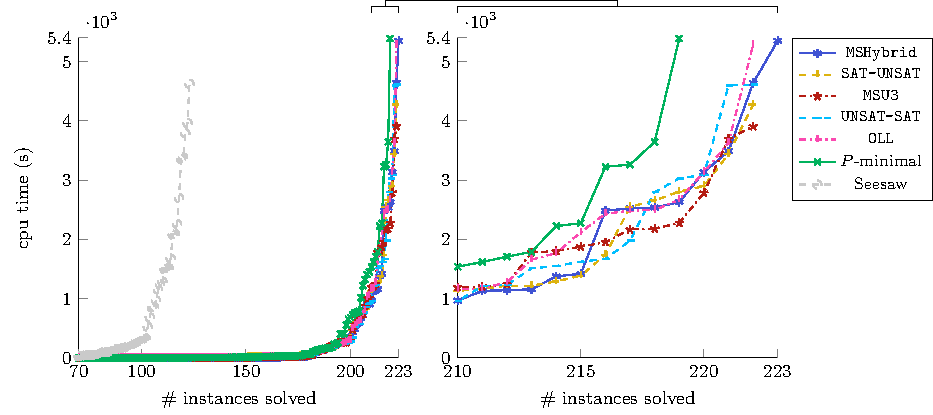
\includegraphics{mlic-cactus-single.pdf}
    \caption{Runtime comparison of  $P$-minimal and variants of \algname{} for LIDR; plot on the right
      is zoomed in on the more interesting part of the left plot.
      %        On the right, a magnified version from 195 solved instances on is shown.
    }\label{fig:mlic-cactus}
\end{figure}

We start with a comparison of the runtime performance of different variants of \algname{}, $P$-minimal and (for LIDR) Seesaw.
For LIDR, \Cref{fig:mlic-cactus} shows the number of instances solved ($x$-axis) for different per-instance time limits ($y$-axis) for the task of
computing a single representative solution for each pareto point.
The best-performing approach is the \algname{} variant \msh{}, solving 223 instances, while $P$-minimal solves 219 instances.
%With that, it outperforms $P$-minimal by four solved instances.
All  variants of \algname{} outperform $P$-minimal to some extent.
Seesaw is very clearly outperformed by all other approaches, solving only 123 instances within the resource constraints.
\Cref{fig:setcover-cactus} shows a similar comparison for the two variants of bi-objective set covering.
Here again \msh{} is the best-performing variant of \algname{}, considerably outperforming $P$-minimal:
$P$-minimal  solves 71 (resp.~38) fixed element probability (resp., fixed set cardinality) instances,
whereas \msh{} solves  82 (resp.~40) instances.
Similar plots for the task of enumerating all solutions on the pareto front are provided in Appendix~\ref{sup:plots}.

\begin{figure}
    \centering
    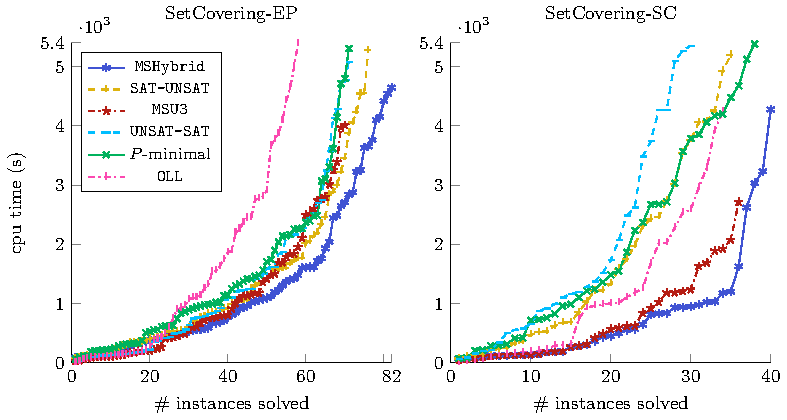
\includegraphics{setcover-cactus-single.pdf}
    \caption{Runtime comparison of $P$-minimal and variants of \algname{} for  bi-objective set covering problem.
      %The plot on the left is over instances generated with fixed probability that an element is in a set while the plot on the right is for instances with fixed set cardinality.
    }\label{fig:setcover-cactus}
\end{figure}

%Next, we compare \algname{} with $P$-minimal on  bi-objective set covering; see
%\Cref{fig:setcover-cactus} for a runtime comparison for
% fixed element probability instances (left) and fixed set cardinality instances (right).
% $P$-minimal  solves 71 (resp., 38) fixed element probability (resp., fixed set cardinality) instances,  while the best-performing \algname{} variant (\msh{}) solves
% 82 (resp., 40).

\begin{table}
  \centering
  \caption{Solved instances by approach and benchmark family.
%      The numbers are provided for computing a \emph{single} representative solution per pareto point or \emph{all} of them.
      %        The best approach per instance is highlighted in bold.
  }\label{tab:nsolved}
  \begin{tabular}{@{}lr@{\hskip 3pt}rr@{\hskip 3pt}rr@{\hskip 3pt}rr@{\hskip 3pt}rr@{\hskip 3pt}rr@{\hskip 3pt}r@{}}
    \toprule
    \multirow{2}{*}{Instance Type} & \multicolumn{2}{c}{\satunsat} & \multicolumn{2}{c}{\unsatsat} & \multicolumn{2}{c}{\msu} & \multicolumn{2}{c}{\oll} & \multicolumn{2}{c}{\msh} & \multicolumn{2}{c}{$P$-minimal} \\
    \cmidrule(r){2-3} \cmidrule(r){4-5} \cmidrule(r){6-7} \cmidrule(r){8-9} \cmidrule(r){10-11} \cmidrule(r){12-13}
    & single & all & single & all & single & all & single & all & single & all & {\hskip 6pt}single & all \\
    \midrule
    Decision Rules & 222 & \textbf{215} & 222 & \textbf{215} & 222 & \textbf{215} & 222 & 212 & \textbf{223} & \textbf{215} & 219 & 213 \\
    SetCovering-EP & 76 & 73 & 71 & 71 & 70 & 70 & 58 & 58 & \textbf{82} & \textbf{80} & 71 & 68 \\
    SetCovering-SC & 35 & 29 & 30 & 26 & 36 & 36 & 34 & 34 & \textbf{40} & \textbf{40} & 38 & 26 \\
    \bottomrule
  \end{tabular}
\end{table}

\begin{figure}
    \centering
    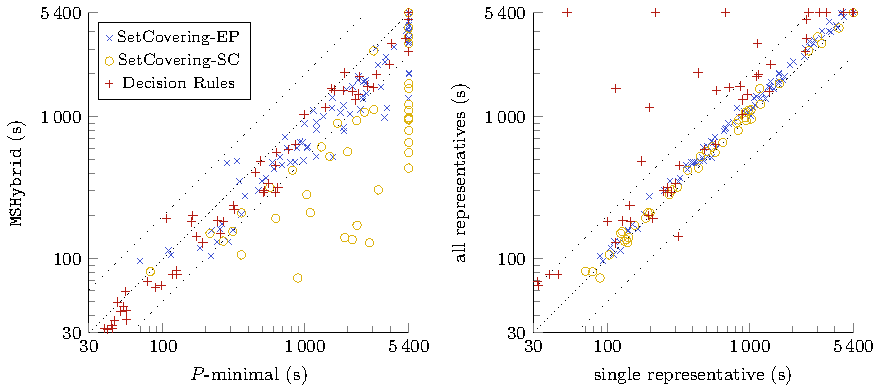
\includegraphics{all-datasets-combined-msh-and-enumeration.pdf}
    \caption{Left: Runtime comparison between $P$-minimal and \algname{} in the \msh{} variant. % over different instance types.
      Right: Runtime comparison between enumerating a single representative vs all solutions per pareto point with \msh{}.
%      point or all pareto-optimal solutions with the \msh{} variant.
      %        Instances with less than 30 seconds runtime are not shown.
    }\label{fig:msh-scatter}
\end{figure}

The numbers of solved instances are summarized in \cref{tab:nsolved},
both for  enumerating a single representative solution per pareto point and for enumerating \emph{all} pareto-optimal solutions.
\msh{} is the best-performing \algname{} variant overall, outperforming $P$-minimal in all cases. The performance difference
is greater when enumerating all pareto-optimal solutions.
For more details,
\cref{fig:msh-scatter} (left) shows a per-instance runtime comparison between \msh{} and $P$-minimal.
%In this plot, the dotted diagonal lines mark equal runtimes as well as double runtime in either direction.
We note that
$P$-minimal did not uniquely solve any instance. In general, \msh{} was outperformed by $P$-minimal on only 37 instances while \msh{} solves 308 instances in less time.
\Cref{fig:msh-scatter} (right) shows a runtime comparison between enumerating a single representative solution per pareto point and enumerating all pareto-optimal solutions with \msh{}.
 Overall, the approach scales well also for the latter task, although there understandably is an overhead 
  when the number of solutions required to be enumerated grows significantly; this is the case for
  LIDR
  where some instances
  have 
  more than $10,000$ solutions per pareto point.
This is in contrast to the set covering instances, which tend to have only a single (or few) solutions per pareto point.
%More details on enumerating all representative solutions with all approaches can be found in \cref{sup:plots}.
%  Since the set covering instances are weighted, and therefore it is significantly less likely that two solutions lead to the same objective values, these instances typically only have a single solution corresponding to every pareto point.
%Therefore, no significant difference in runtimes is visible for enumerating a single compared to all representative solutions.

\begin{figure}
    \centering
    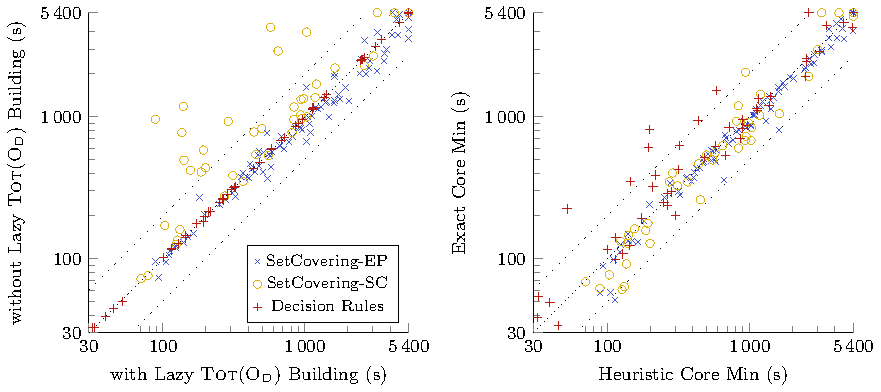
\includegraphics{all-datasets-chosen-refinements.pdf}
    \caption{Instance runtime comparisons for the two refinements lazily building the totalizer for the decreasing objective (left) and exact core minimization (right).
      %        Marker shapes and colours represent different instance types and instances with less than 30 seconds runtime are cropped out.}
      } \label{fig:refinements}
\end{figure}

Finally,
we evaluated the impact of the proposed refinements on the runtime efficiency of the best-performing approach, \msh{}.
%We consider two refinements in detail: lazily building $\tot(\Obj_\dec)$ and exact core minimization.
\Cref{fig:refinements} shows
the impact of lazily building $\tot(\Obj_\dec)$ (left) and exact vs heuristic core minimization (right).
Lazily building $\tot(\Obj_\dec)$ has no evident impact on LIDR,
as expected
(the literals from $\Obj_\dec$ do not appear in $\Obj_\inc$ and $\tot(\Obj_\dec)$ can therefore not be lazily built).
%For the set covering instances generated with fixed element probabilities, we see a slight negative effect for medium runtimes, but we have two instances that could only be solved when lazily building $\tot(\Obj_\dec)$.
For fixed set cardinality set covering, however, we see a strong positive effect.
%This is most likely due to the fact that the instances generated with fixed set cardinalities on average have more elements that don't appear in any of the sets and can therefore be left out of $\tot(\Obj_\dec)$.
Heuristic core minimization appears to have a positive effect  on LIDR as well as on harder set covering instances,
although the difference to exact minimization is smaller
than that of lazily building $\tot(\Obj_\dec)$.
%For set covering, exact core minimization has a slightly positive effect for instances that are solved in less time, for instances with long runtimes however, the effect is slightly negative.
%
%Other than those refinements, we also evaluated adding a
%The third refinement, i.e., disjoint phase to \msu{} which we found to have no lead to an improvement in performance.
%Data on this claim can be found in \cref{sup:plots}.
\include{Ch.50_Conclusions}

%%%%%%%%%%%%%%%%%%%%%%%%%%%%%%%%%%%%%%%%%%%%%%%%%%%%%%%%%
%\cleardoublepage                          %fixes the position of bibliography in bookmarks
%\phantomsection
\addcontentsline{toc}{chapter}{\bibname}  % This lines adds the bibliography to the ToC
\printbibliography

%%%%%%%%%%%%%%%%%%%%%%%%%%%%%%%%%%%%%%%%%%%%%%%%%%%%%%%%%
\backmatter
\begin{appendices}

%% A sample Appendix
\include{Ch.90_Appendix_1}

\end{appendices}
%%%%%%%%%%%%%%%%%%%%%%%%%%%%%%%%%%%%%%%%%%%%%%%%%%%%%%%%%

\end{document}
